\subsection{Математическая модель №1}
\label{subsec:mathmodel_1}

\subsubsection{Цепь Маркова}
\label{subsubsec:markovchain_1}
Представим $\Tin/\Tres$ в виде несократимой дроби $\tin/\tres$, где $\tin, \tres\in\mathbb{N}$. Назовем слотом интервал времени длины $$\tau \equiv  \frac{\Tin}{\tin} = \frac{\Tres}{\tres}.$$ Разобьем непрерывную временную шкалу на слоты таким образом, чтобы начало каждого зарезервированного интервала совпадало с началом некоторого слота -- см.~рис~\ref{fig:time}.

Процесс передачи пакетов с помощью механизма периодических резервирований может быть описан цепью Маркова с дискретным временем, единица которого равна периоду резервирований.

\begin{figure}[t]
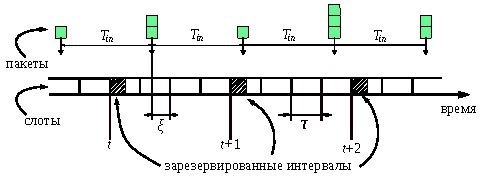
\includegraphics[width=\linewidth]{MarkChain.pdf}
\caption{\label{fig:time} Слотированное время}
\end{figure} 

В каждый момент времени $t$ состояние системы будем описывать парой целых чисел $(h(t), m(t), n(t))$. Если $h(t) \geqslant 0$, то очередь не пуста, и $h(t)$ равно числу полных слотов, которые головная (самая старшая) пачка пакетов провела в очереди, $m(t)$ равно числу пакетов в этой пачке, а $n(t)$ равно начальному числу пакетов в головной пачке. Если $h(t) < 0$, то очередь пуста, и $|h(t)|$ равно времени до прибытия новой пачки пакетов, выраженному в слотах и округленному вниз; при этом $m=n$, а $n$ задаётся случаным образом, исходя из распределения $\{ p_{ij} \}_{i=1, j=1}^{i=M, j=M}$ и начальным размером предыдущей головной пачки. Это значит, что в любой момент времени $m(t) > 0$. Таким образом, состояние системы в каждый моменты времени $t$ характеризуется текущим числом пакетов в головной пачке, начальным числом пакетов  в головной пачке и временем, в течение которого пакеты этой пачки ожидают передачи. Используемые обозначения состояния системы позволяют определить количество пачек пакетов в очереди, ($\lfloor h(t)/\tin \rfloor + 1$ в момент времени $t$), но не позволяют определить длины всех пачек, кроме головной. После того, как все пакеты головной пачки были переданы или отброшены, определяется число пакетов в пачке, ставшей головной.
  
Минимальное значение $h(t)$ равно $\tres-\tin$. Оно достигается в момент времени $t$, если пачка из одного пакета пребывает в пустую очередь непосредственно перед моментом $t - 1$, и единственный пакет пачки успешно передается с первой попытки.   

Теперь найдем максимальное возможное значение $h(t)$. Для этого обозначим через $\xi$ время между поступлением пачки пакетов в очередь и началом следующего слота, $0 \leqslant \xi < \tau$. В силу того, что время $\Tin$ равно целому числу $\tin$ слотов, значение величины $\xi$ одинаково для всех пачек. Таким образом, к моменту времени $t$ время ожидания в очереди пакетов головной пачки равно $h(t) \cdot \tau + \xi$. Чтобы эта пачка не была отброшена в момент $t$, ее время ожидания не должно превышать значения $D$. Следовательно, $h(t) \leqslant d = \lfloor \frac{D-\xi}{\tau} \rfloor$. 

Благодаря тому, что числа $\tin$ и $\tres$ взаимно просты, цепь Маркова обладает свойством эргодичности. Таким образом, может быть найдено стационарное распределение вероятностей цепи Маркова. 

Выясним, в какие состояния и с какой вероятностью может перейти система из состояния $(h, m, n)$ за один шаг. Для этого отдельно рассмотрим несколько случаев.

\paragraph{1.} Пусть $h < 0$. Тогда на данный момент очередь пуста, значит, система перейдёт в состояние $(h + \tres, m, m)$.

\paragraph{2.} Пусть $d - \tres< h$. Тогда очередь не пуста, но к моменту начала следующего интервала резервирования истечёт время $\DQoS$ ожидания пакетов в головной пачке к моменту времени $t + 1$ система окажется в состоянии $(h + \tres - \tin, i, i)$ с вероятностью $p_{ni}$. Однако, следует учесть, что в этом случае с вероятностью $\qdet p_{ni}$ было потеряно $m$ пакетов, поскольку попытка передачи была неуспешной, а с вероятностью $(1 - \qdet) p_{ni}$ --- $m - 1$ , $i \in \{ 1, \ldots, M \}$. 

\paragraph{3.} Пусть $0 \leq h \leq d - \tres$. Тогда очередь не пуста, и к моменту времени $t + 1$ система окажется в состоянии:
\begin{itemize}
\item $(h + \tres, m, n)$ с вероятностью $\qdet$ в случае неудачной попытки передачи.
\item в случае удачной попытки передачи:
	\begin{itemize}
	\item $(h - \tin + \tres, i, i)$ с вероятностью $(1 - \qdet)p_{ni}$, если $m(t) = 1$;		
	\item $(h + \tres, m - 1, n)$ с вероятностью $(1 - \qdet)$, если  $m(t) > 1$.
	\end{itemize}
\end{itemize}

\paragraph{Подводя итог,} получаем, что при выполнении соответствующих условий система  переходит из состояния $(h, m, n)$ в одно из следующих состояний:

\begin{tabular}{l l l l}
1)	&$(h + \tres, m, m)$,	&$\gamma = 1$,	&при $h < 0$;\\
2)	&$(h + \tres - \tin, i, i)$,	&$\gamma = p_{ni}$,	&при $d - \tres< h$;\\
3)	&$(h + \tres, m, n)$,	&$\gamma = \qdet$,	&при $0 \leq h \leq d - \tres$;\\
4)	&$(h - \tin + \tres, i, i)$,	&$\gamma = ( 1 - \qdet) p_{ni}$,	&при $m = 1$, $0 \leq h \leq d - \tres$;\\
5)	&$(h + \tres, m - 1, n)$,	&$\gamma = ( 1 - \qdet)$,	&при $m > 1$, $0 \leq h \leq d - \tres$;\\
\end{tabular} \newline
где $i\in\{1,\ldots,M\}$ и $\gamma$ --- вероятность перехода. 

\subsubsection{Определение PLR}
Упорядочив состояния в лексикографическом порядке и построив матрицу $P$ переходных вероятностей, найдем стационарные вероятности $\pi_{(h,m,n)}$ состояний $(h,m,n)$.

Зная станционарные вероятности $\pi_{(h,m, n)}$, найдем долю $PLR$ потерянных пакетов. Так как пакеты отбрасываются только при превышении порога времени $\DQoS$ ожидания в очереди, потери пакетов могут происходить только при переходе $2$. Как упоминалось ранее, в случае успешной попытки передачи будет потерян $m - 1$ пакет, в ином случае --- $m$ пакетов. Тогда среднее число пакетов, отбрасываемых за один шаг модельного времени ($\Tres$), равно
$$
	\Idis = \sum\limits_{(h,m, n)\colon h > d - \tres} \left((m - 1)(1 - \qdet)\pi_{(h,m,n)} + m\qdet\pi_{(h,m,n)}\right) = \\
	=\sum\limits_{(h,m,n)\colon h > d - \tres} (m - 1 + \qdet)\pi_{(h,m,n)}.
$$

Значение $PLR$ равно отношению среднего числа $\Idis$ пакетов, отброшенных за один шаг модельного времени, к среднему числу $\Iin$ пакетов, поступивших в очередь за то же время:
$$
PLR = \frac{\Idis}{\Iin} = \frac{1}{\frac{\Tres}{\Tin} \sum\limits_{i} i\cdot p_i} \cdot \left(\sum\limits_{(h,m,n)\colon h > d - \tres} (m - 1 + \qdet)\pi_{(h,m,n)} \right).
$$